%!TEX root = ../../../thesis.tex

Details of components in the electrode-electrolyte interface model and methods of determining its parameters have been discussed.
The focus now moves to measuring and fitting of the model parameters to the model.
Model parameters will first be determined for various concentrations of phosphate buffered saline (PBS), and then for comparison -- in a living sheep's spinal cavity.
This tells us whether a one-tenth concentration of PBS is in-fact a good substitute for cerebrospinal fluid (CSF), which it is assumed to be by implant engineers.

\section{Phosphate Buffered Saline}
    Scott \& Single fitted parameters of their model to a one-tenth concentration (0.1X) of a standard solution of PBS \cite{Scott2014}.
    I measure and fit parameters not only to the one-tenth concentration of PBS but to a range of concentrations from 0.025X up to 1X.
    Not all of the model parameters vary with concentration, but for the ones that do, a fit of the parameter's value to concentration using regression analysis has been made. %TODO: Correct punctuation in this sentence?%
    Doing this gives a a model that can be used to predict the impedance response of an electrode array in a wide range of solution concentrations.

    Each of the PBS measurements were made in \SI{1}{\litre} glass bottles containing \SI{700}{\milli\litre} of PBS solution in each case.
    Measurements were made in a controlled environment maintaining an ambient temperature of \SI{23}{\degree} Celsius.
    All measurements were automated by the use of Python scripts running on a GNU/Linux based workstation.
    The scripts communicate with the instruments both to configure measurements and collect data.
    Each measurement set was repeated for each of the six concentrations of PBS used.
    % The six concentrations of PBS measured are 0.025X, 0.05X, 0.1X, 0.25X 0.5X, and 1.0X the concentration of the standard stock solution.
    The six concentration of PBS measured are shown in \cref{tab:pt2-PBS_concentrations}.
    \begin{table}
      \centering
      \begin{tabular}{l}
        Concentration\\
        \hline
        1.00X\\
        0.5X\\
        0.25X\\
        0.1X\\
        0.05X\\
        0.025X\\
      \end{tabular}
      \caption{\label{tab:pt2-PBS_concentrations}Six PBS concentrations used to fit model parameters to.}
    \end{table}

    \subsection{Resistor Mesh}

      \begin{figure}
        \centering
        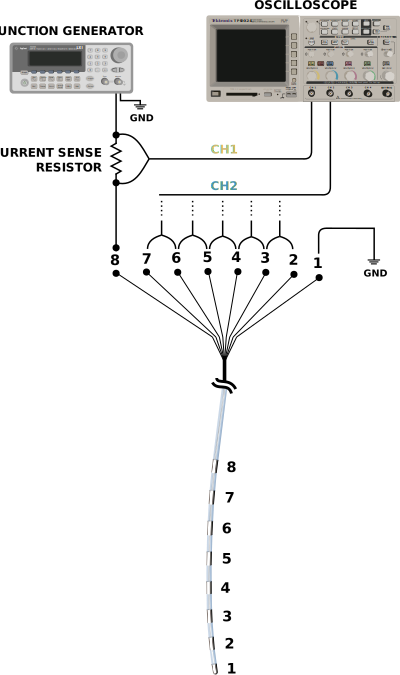
\includegraphics{content/pt2/08-InterfaceParameters/graphics/measurement_resistorMesh}
        \caption{\label{fig:pt2-measurement_resistorMesh}Illustration of one of two measurement configurations used to to measure the electrode transimpedances. Each of the electrode pairs were measured one-after-the-other using the shown equipment.}
      \end{figure}

      With the electrode immersed in a solution of PBS a \SI{10}{\kilo\hertz} sinusoidal current having an amplitude of \SI{500}{\micro\ampere} was passed through the stimulus electrodes using an Agilent 33220A function generator.
      A current sense resistor was inserted in series with the stimulus electrodes.
      The differential voltage across a pair of non-stimulating electrodes and the voltage across the current sense resistor was measured using a Tektronix TPS 2024 oscilloscope.
      \Cref{fig:pt2-measurement_resistorMesh} shows the measurement configuration used when electrodes one and eight are used as the stimulus electrodes.
      The second configuration has electrodes 8 and 7 as stimulus electrodes and the remaining electrode pairs are used to measure transimpedance voltage differentials.

      \begin{figure}
        \centering
        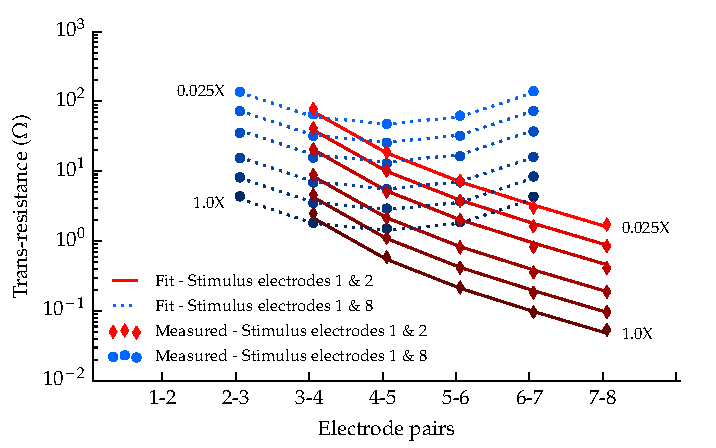
\includegraphics{content/pt2/07-InterfaceModel/graphics/graph_transimpedance_pbs}
        \caption{\label{fig:pt2-graph_transimpedance_pbs}Measured and fitted values of trans-impedance for both measurement configurations. Voltage measurements are made between adjacent pairs of electrodes as current is pushed through the stimulus electrodes.}
      \end{figure}
      The results of those measurements, in both configurations, are shown by markers in \cref{fig:pt2-graph_transimpedance_pbs}.
      Each point is calculated by taking the voltage differential across a pair of electrodes ($V_{diff}$) and dividing by the stimulus current of \SI{500}{\micro\ampere}.
      \begin{table}
        \centering
        \begin{tabular}{r | l}
          Parameter & Value \\
          \hline
          $R_{eri}$ ($\Omega$)& 0.407 / $\sigma$\\
          $R_{sri}$ ($\Omega$)& $R_{eri}\cdot 3/4$\\
          $R_{li}$ ($\Omega$)& 3.71 / $\sigma$ \\
          Depth (layers) & 5 \\
          Padding (layers) & 3 \\
        \end{tabular}
        \caption{\label{tab:RESparams}Resistor mesh parameters. Electrolyte conductivity ($\sigma$) is expressed in units of $S / cm$.}
      \end{table}

      Values for $R_{eri}$ and $R_{li}$ are using a custom Python optimisation script employing the NumPy library for each concentration of PBS.
      The optimisation script selects candidate values for $R_{eri}$ and $R_{li}$, simulates the mesh using those values, and then calculates the equivalent trans-impedance values.
      The error between simulated trans-impedance values and measured values is calculated and the process repeats, selecting different values of $R_{eri}$ and $R_{li}$ to improve the fit.
      The final values of $R_{eri}$ and $R_{li}$ are those that minimise the error, they are shown in \cref{tab:RESparams}.
      $R_{sri}$ is a dependent variable, so is expressed in terms of $R_{eri}$, and the remaining parameters have been re-used from the work of Scott \& Single.
      \Cref{fig:pt2-graph_transimpedance_pbs} shows measurement results for each pair of non-stimulated pair of electrodes along with simulated results using the fitted parameters.


    \subsection{Series Resistance And Constant Phase Element}
      \begin{figure}
        \centering
        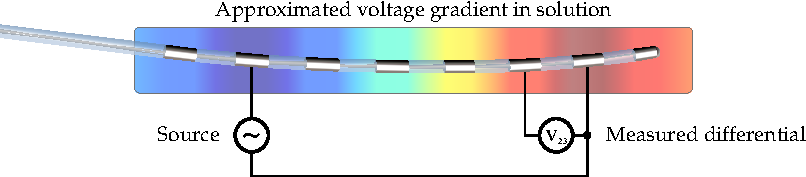
\includegraphics{content/pt2/08-InterfaceParameters/graphics/measurement_CPE}
        \caption{\label{fig:pt2-measurement_CPE}Illustrated voltage gradient in electrolyte solution at each electrode's surface when potential is applied across electrodes two and seven. Measurement of electrolyte voltage taken between electrodes 2 and 3.}
      \end{figure}
      Measurement of both the CPE and the interface's series resistance is made using impedance spectroscopy methods.
      A sinusoidal current is passed between electrodes two and seven of the electrode array.
      Use of the end electrodes (one and eight) was avoided as a precaution to reduce end effects.
      The sinusoidal voltage at the liquid side of the interface is taken as the the voltage that appears at an adjacent electrode (electode three) when a suitably high impedance measurement is made, this is illustrated in \cref{fig:pt2-measurement_CPE}.
      This measurement relies on the ability to make high impedance voltage measurements to minimise voltage drop across the electrode interface, for which a Tektronix TPS 2024 four channel oscilloscope was used.
      All four of its channels are floating and have an input resistance of \SI{10}{\mega\ohm} using 10X probes.
      An Agilent 33220A Function Generator was used to generate the stimulus waveforms applied between electrodes two and eight.
      A series resistance of \SI{10}{\kilo\ohm} was inserted in series with the waveform generator's output.
      It serves as a current sense resistor, also measured using the oscilloscope.
      \begin{figure}
          \centering
          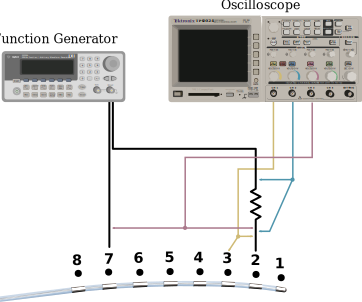
\includegraphics[scale=0.95]{content/pt2/08-InterfaceParameters/graphics/measurement_CPE_setup}
          \caption{\label{fig:pt2-measurement_CPE_setup}Diagram showing the measurement configuration used to measure the CPE response and interface series resistance.}
      \end{figure}
      By measuring the current through electrode two and the voltage across electrodes two's interface, the impedance of the interface can be calculated.
      A diagram showing the measurement setup is shown as \cref{fig:pt2-measurement_CPE_setup}.
      For each of the six solutions, twenty frequencies (log-spaced) were sampled between \SI{50}{\milli\hertz} and \SI{10}{\kilo\hertz} for the impedance measurements.
      At each frequency the stimulus waveform amplitude was re-adjusted to be \SI{300}{\milli\volt}-peak as the interface's impedance changed.
      \begin{figure}
        \centering
        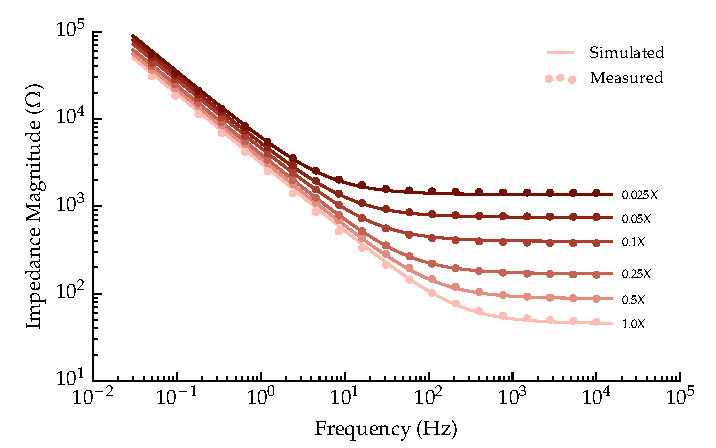
\includegraphics{content/pt2/08-InterfaceParameters/graphics/displacement_impedanceVsFrequency_magnitude_thesis}
        \caption{\label{fig:pt2-graph_impedanceVsFrequency_magnitude}Impedance magnitude of both the measured interface response and the fitted response at each of the six concentrations of PBS.}
      \end{figure}
      \begin{figure}
        \centering
        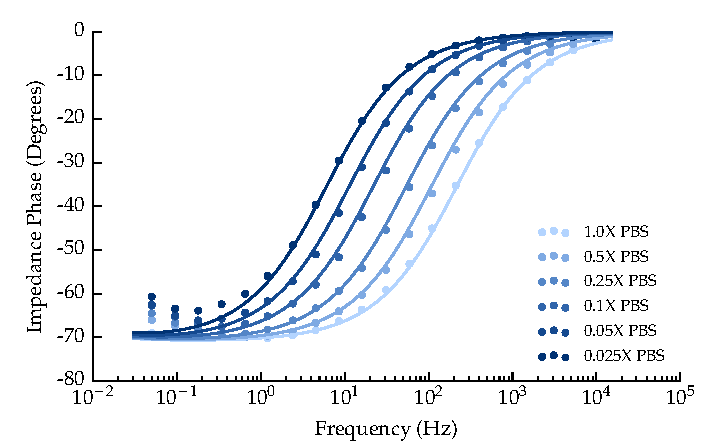
\includegraphics{content/pt2/08-InterfaceParameters/graphics/displacement_impedanceVsFrequency_phase_thesis}
        \caption{\label{fig:pt2-graph_impedanceVsFrequency_phase}Impedance phase of both the measured interface response and the fitted response at each of the six concentrations of PBS.}
      \end{figure}
      \Cref{fig:pt2-graph_impedanceVsFrequency_magnitude,fig:pt2-graph_impedanceVsFrequency_phase} show the calculated impedance magnitude and phase from measurements as markers and simulation results of the fitted parameters as traces.
      \begin{figure}
        \centering
        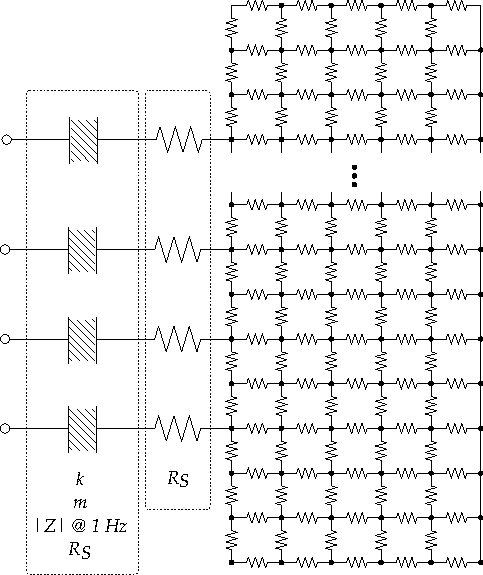
\includegraphics{content/pt2/08-InterfaceParameters/graphics/SpiceModel_opitimisation}
        \caption{\label{fig:pt2-spiceModel_optimisation}The SPICE model schematic used to find optimum values for parameters of the CPE and interface series resistance. Parameters for the resistor mesh are those determined previously.}
      \end{figure}
      \Cref{fig:pt2-spiceModel_optimisation} shows the SPICE model used to simulate parameter values for the CPE and $R_{s}$.
      Final values were found by minimising the difference between the simulated response and the measured response using a Python script.
      For each set of parameter values in the optimisation the script builds a SPICE circuit using those parameter values, simulates the circuit, calculates the interface impedance and compares the values to the measured results.
      The process is automated and runs until a minimum error between simulated and measured results is found.
      Once found, the script exists and displays the final values of each parameter.
      After parameter values are found for each concentration of PBS, another optimisation is made to scale relevant parameters by the concentration.
      The parameters that are scaled with concentration are the series resistance ($R_{S}$) and the CPE's impedance magnitude at \SI{50}{\milli\hertz}.
      The final fit expresses these parameters as functions dependent on the concentration of PBS.
      \begin{figure}
        \centering
        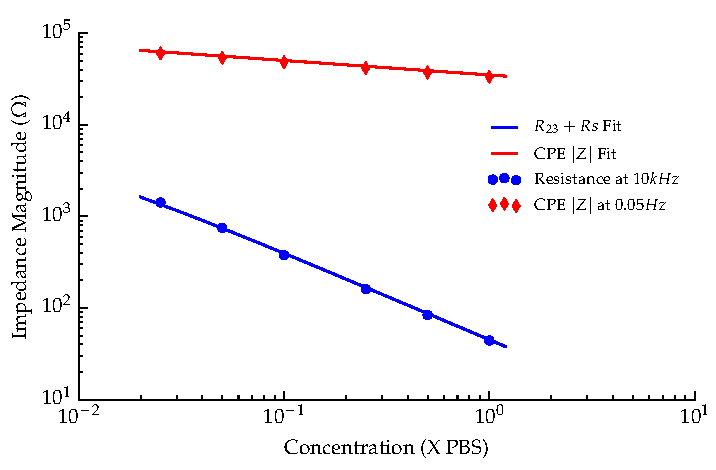
\includegraphics{content/pt2/08-InterfaceParameters/graphics/scalingFactors_Displacement_Thesis}
        \caption{\label{fig:pt2-scalingFactors_Displacement_Thesis}Plot showing fitted parameter values for the CPE impedance magnitude at \SI{50}{\milli\hertz} and series resistance at each of the six concentrations of PBS (shown as markers). The solid trace shows the resulting fit between those values as a function of concentration.}
      \end{figure}
      Individual parameter values for each concentration, along with the resulting fit, is shown in \cref{fig:pt2-scalingFactors_Displacement_Thesis}.
      Measurements of the CPE's vertical position were made at \SI{50}{\milli\hertz}, as opposed to the parameters defined value at \SI{1}{\hertz}, to avoid any effect from the series resistance interfering with the measured value.
      As the slope of the CPE is always the same, the value can be easily converted back to the equivalent value at \SI{1}{\hertz}.
      Measured resistance at high frequency includes the inter-electrode resistance ($R_{23}$) which has been included in the plot, but will be subtracted to leave only $R_{S}$.
      \begin{table}
        \centering
        \begin{tabular}{r | l}
          Parameter & Value \\
          \hline
          $m$& 1.34\\
          $k$ & 1.773\\
          |Z| @ \SI{1}{\hertz} ($\Omega$)& $3284 \times concentration^{-0.158}$ \\
          $R_{S}$ ($\Omega$)& $13.38 \times concentration^{-0.8397}$
        \end{tabular}
        \caption{\label{tab:CPEparams}CPE and $R_{s}$ parameters. Concentration is relative to the stock solution of phosphate buffered saline.}
      \end{table}
      The final parameters for the CPE and $R_{S}$ are given in \cref{tab:CPEparams}.

    \subsection{Faradaic Current}
      \begin{figure}
        \centering
        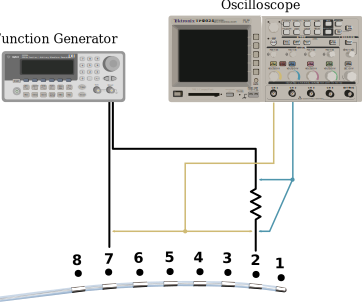
\includegraphics{content/pt2/08-InterfaceParameters/graphics/measurement_Faradaic_setup_initial}
        \caption{\label{fig:pt2-measurement_Faradaic_setup_initial}Illustration of the cyclic voltammetry measurement configuration used to measure the response of the interface when driven into Faradaic conduction mode.}
      \end{figure}
      Using the same oscilloscope and function generator as the previous measurement, the oscilloscope is set to measure voltage between electrodes two and seven and the current through the current sense resistor.
      The function generator is set to produce a triangle wave stimulus, or linear ramp, also between electrodes two and seven.
      Electrical current associated with Faradaic reactions rises exponentially after a certain electrode overpotential.
      The point at which the electrical current draw begins to move exponentially with increasing voltage represents the onset of the associated reaction.
      \begin{figure}
        \centering
        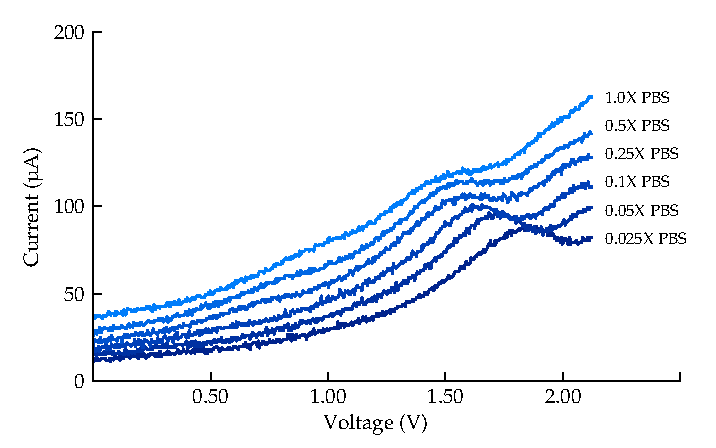
\includegraphics{content/pt2/08-InterfaceParameters/graphics/faradaicOnset-all-average}
        \caption{\label{fig:pt2-faradaic_measurement}Graph showing measured Faradaic response of each concentration of PBS to a linearly increasing voltage between electrodes two and seven.}
      \end{figure}

      \Cref{fig:pt2-faradaic_measurement} shows measured data where the Faradaic response is evident for each concentration.
      The repeatability of these measurements was low although care was taken to recreate the same conditions for each run.
      To try and improve the repeatability the following was tried:
      \begin{itemize}
        \item Maintaining a constant ambient temperature
        \item Cleaning the electrodes between each measurement using isopropyl alcohol
        \item Keeping the electrolyte moving at a constant velocity using a motorised stirrer
        \item Letting the system to settle for periods up to two hours between measurements
      \end{itemize}
      These steps reduced variation between measurements, but by no means removed the variation.
      Sweeping the voltage at \SI{0.12}{\volt\per\second} was slow enough that results did not appear to be too distorted but fast enough that a measurement run could be completed quickly.
      Completing measurements quickly seemed important at the time as it was often the case that an artifact would show up during a measurement run, for what seemed like no apparent reason, and affect the remainder of the experiments.
      Artifacts were sometimes a peak at a certain voltage, otherwise they would manifest themselves as distortions to the current/voltage trace.
      A key insight was realising that after the voltage across a pair of electrodes had been pushed into Faradaic region they then began to behave differently, even after being returned to lower stimulus voltages.
      In \cref{fig:pt2-faradaic_measurement} it is clear that each concentration has a different Faradaic response.
      This means that when the maximum voltage is applied to each of the solutions that the highest concentration is driven further into its Faradaic region that the rest.
      That in turn would create an artifact that would appear on the remaining traces (those of lower concentration), that would not have otherwise been there.
      The issue of artifact and dependence on sweep rate led me to find other ways of measuring Faradaic currents.

      \subsubsection{Step based Faradaic measurements}
        \begin{figure}
          \centering
          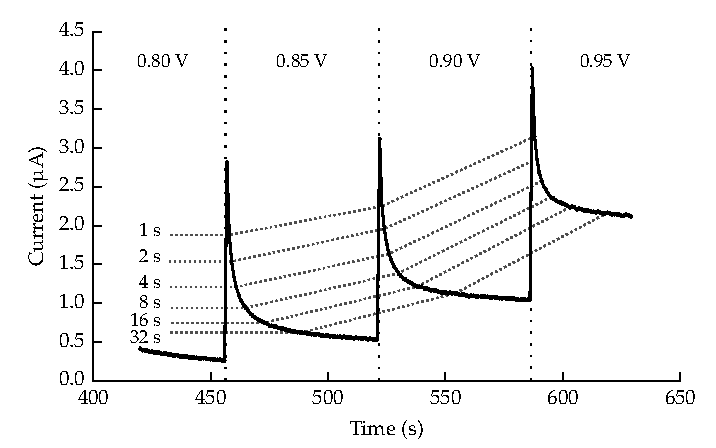
\includegraphics{content/pt2/08-InterfaceParameters/graphics/graph_64s_stirred}
          \caption{\label{fig:pt2-faradaic_decay}Graph showing measured response of two interfaces to a multiple step responses. Vertical dotted lines indicate when in time the step occurred. Dotted traces show points in time after each response. Measurements are between electrodes two and seven on the Octrode submerged in 1X PBS.}
        \end{figure}

        A revealing measurement came from the use of the Agilent E5270B precision measurement mainframe, the same instrument that was used to measure the streaming potential cells.
        By increasing the voltage between the electrodes in discrete steps and recording the current over time it became clear that the CPE was having a large effect on measurement results.
        \Cref{fig:pt2-faradaic_decay} shows three transitions in steps of \SI{0.05}{\volt} occurring \SI{64}{\second} apart.
        The dotted traces show what the result would be if the measurement were taken at that time, i.e. the trace would take the shape of the dotted line of the corresponding delay time.
        This graph shows the effect the CPE is having on measurement results, as well as the duration of time necessary for the transient response to settle.

        \begin{figure}
          \centering
          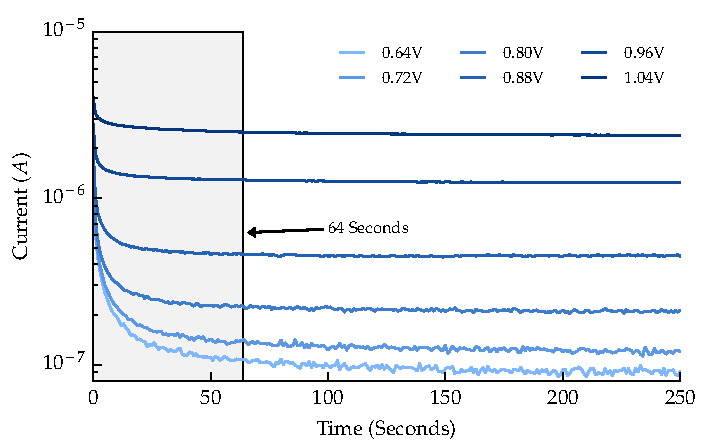
\includegraphics{content/pt2/08-InterfaceParameters/graphics/graph_CPE_currentVsTime_thesis}
          \caption{\label{fig:graph_CPE_currentVsTime}Graph showing CPE discharge curve after a step transition between each of voltage trace in increasing order. Measurements are between electrodes two and seven on the Octrode submerged in 1X PBS. A delay of 10 000 seconds elapsed between each step.}
        \end{figure}
        Subsequent measurements of CPE settling time show that a delay of \SI{64}{\second} between steps is adequate to allow the CPE voltage to settle.
        These measurements are shown as \cref{fig:graph_CPE_currentVsTime}, with the \SI{64}{\second} window highlighted in grey.
        It is interesting to note from these measurements that the capacitance appears to be a function of the applied overpotential, with lower potentials resulting in larger capacitance.

        \begin{figure}
          \centering
          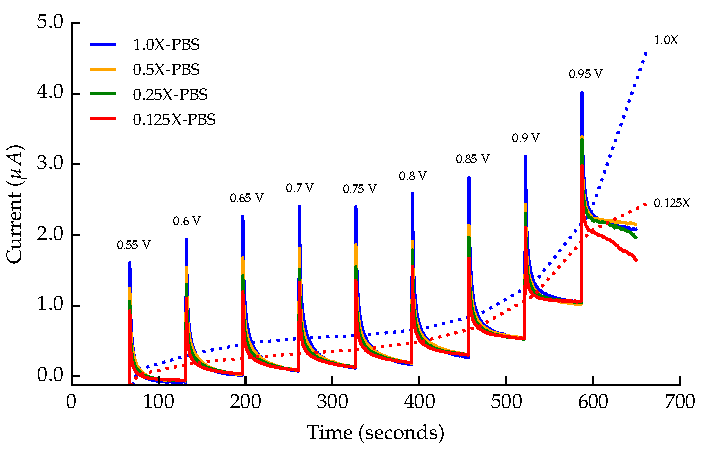
\includegraphics{content/pt2/08-InterfaceParameters/graphics/graph_currentTimeFaradaicCPE_Stacked_Thesis}
          \caption{\label{fig:graph_currentTimeFaradaicCPE_Stacked_Thesis}Graph showing measurements of four concentrations of PBS as each is stepped from \SI{0.55}{\volt} to \SI{0.95}{\volt}. Measurements are between electrodes two and seven on the Octrode. A delay of 64 seconds elapsed between each step. Dotted traces connect current measurements taken \SI{10}{\second} after each step.}
        \end{figure}
        \Cref{fig:graph_currentTimeFaradaicCPE_Stacked_Thesis} shows measurements of four concentrations of PBS overliad on top of one another.
        This graph reveals that not only does the capacitance vary with applied voltage, as was shown in \cref{fig:graph_CPE_currentVsTime}, but also with concentration of PBS.
        A consequence of this is that not waiting long enough to sample the current gives the impression that a higher concentration of PBS results in larger Faradaic currents.
        This is shown by the dotted trace that is sampled \SI{10}{\second} after each step, which I would argue is somewhat representative of cyclic voltammetry measurements.
        Importantly -- the settled current draw for each concentration is approximately the same.
        Any separation between concentrations at the sixty-four second mark for each step appear to be completely random.

        \subsubsection{Successful measurement of the Faradaic currents}
        \begin{figure}
          \centering
          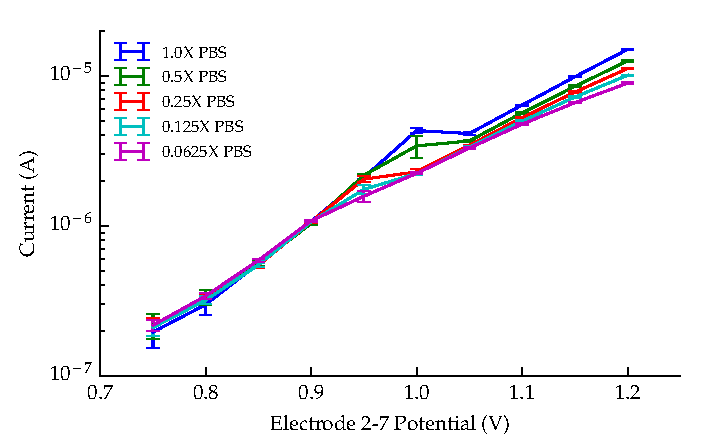
\includegraphics{content/pt2/08-InterfaceParameters/graphics/graph_currentVoltage_logY_Thesis}
          \caption{\label{fig:graph_currentVoltage_logY_Thesis}Graph showing the electrical current draw associated with Faradaic reactions versus applied electrode overpotential. Measurements used the stepped method with a wait time of \SI{64}{\second} between transitions. Vertical bars mark the standard deviation of the final fourty measurements before the following step.}
        \end{figure}
        \Cref{fig:graph_currentVoltage_logY_Thesis} shows the collected measurements of the electrical current due to Faradaic reactions using the stepped measurement method.
        Spread in the measurements at low voltages is due to noise in the measurement samples.
        There are three important observations that can be made from this graph:
        \begin{enumerate}
          \item The effect saline concentration below \SI{0.9}{\volt} has little to no significance on the Faradaic current draw.
          \item Saline concentration is directly related to Faradaic current draw above \SI{1.05}{\volt}.
          \item Between \SI{0.9}{\volt} and \SI{1.05}{\volt} each trace transitions to a mode of saline concentration dependence in reverse order of saline concentration.
        \end{enumerate}

        % I hypothesise that below 1.05
        % I attribute the behaviour seen in \cref{fig:graph_currentVoltage_logY_Thesis} between \SI{0.9}{\volt} and \SI{1.05}{\volt} to a transition from non-limited reactino to a diffusion controlled reaction.

















      % TODO: Write this up in an Appendix
      % \begin{figure}
      %   \centering
      %   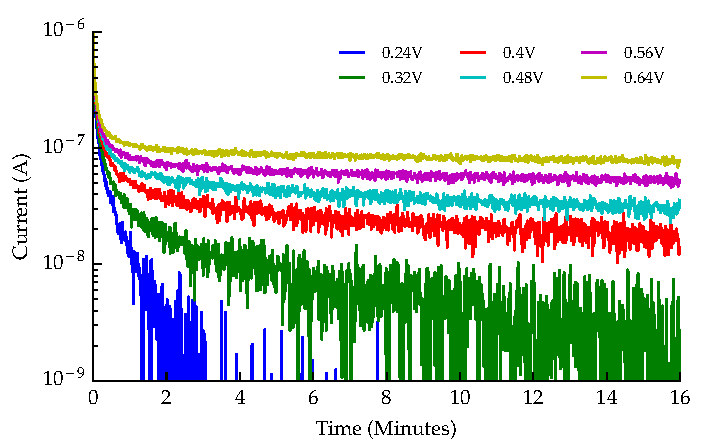
\includegraphics{content/pt2/08-InterfaceParameters/graphics/graph_longsweep_CPE}
      %   \caption{\label{fig:graph_longsweep_CPE}Graph showing current between two electrodes after the voltage is stepped to each of the shown voltages. The total settling time between transition was \SI{10000}{\second}.}
      % \end{figure}




    \subsection{Final Model}

\section{Biological parameter measurements}
    \label{sect:sheep_measurements}
    \subsection{Resistor Mesh}
    \subsection{Series Resistance And Constant Phase Element}
    \subsection{Faradaic Current}
    \subsection{Final Model}
